\section{\large シミュレーション手法}
\subsection{Smoothed Profile Method}
\par 固液二相シミュレーションにおいて,固体-液体の移動界面の取り扱いが非常に重要である.今回のシミュレーションでは,計算手法として流体や粒子の運動について極力近似を用いずに直接数値計算を可能にしたSmoothed Profile Method(SPM)\cite{spm}を用いる.
SPMは,粒子の固体-液体界面にFig. \ref{spm1}のような界面幅$\xi$ に応じた滑らかな界面関数$\phi$を導入することで,境界条件を界面近傍での体積力に変換することで,固液界面において境界条件を解く必要がなくなり,効率の良い直接数値計算を実現し計算時間の短縮が可能となっている.この界面関数を導入することで,系全体をNavier-Stokes方程式で連続的に解くことが可能になる.
\begin{figure}[H]
\centering
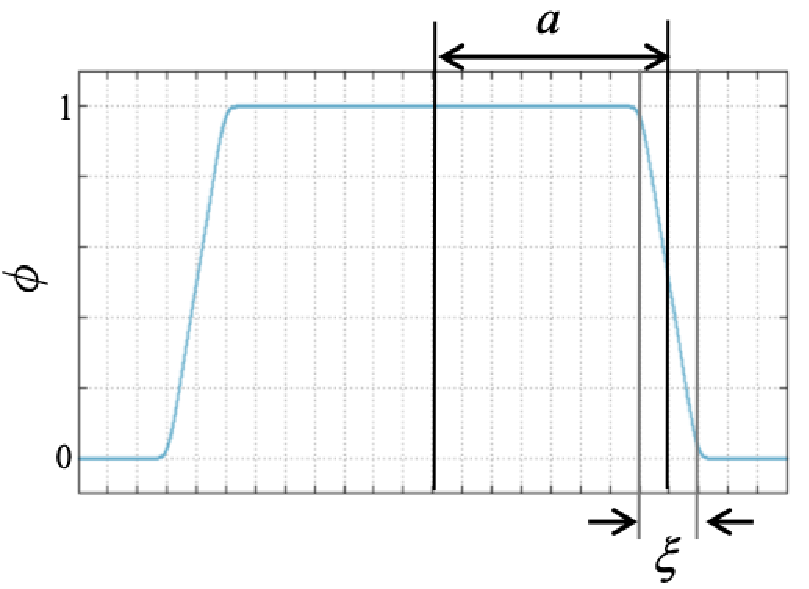
\includegraphics[scale = 0.7]{figures/spm1.pdf}
\caption{Smoothed Profile Method}
\label{spm1}
\end{figure}
%
\begin{figure}[H]
\centering
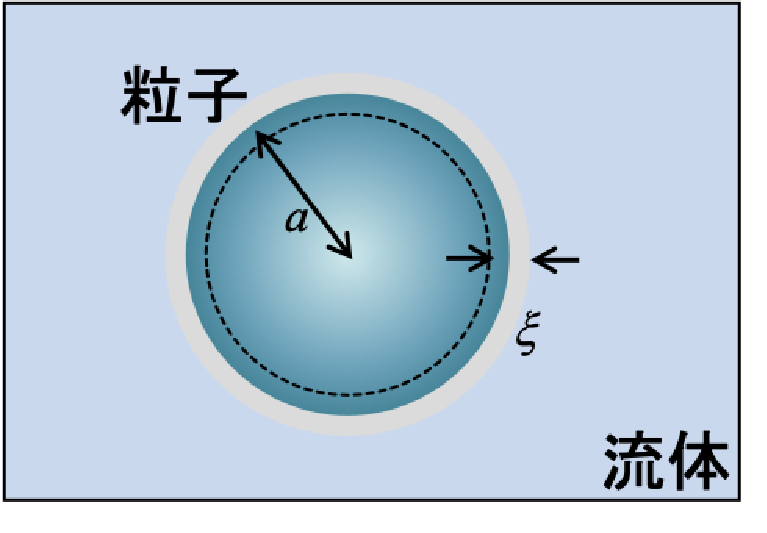
\includegraphics[scale = 0.7]{figures/spm2.pdf}
\caption{界面関数を導入した粒子のイメージ図}
\end{figure}
%	
\newpage
%
\subsection{支配方程式}
\par 本手法では,流体を非圧縮条件のNavier-Stokes方程式,イオンを移流拡散方程式,粒子をNewton方程式及びEuler方程式で解く.
\subsubsection{Navier-Stokes方程式}
%
\vspace*{-2.5zh}
%
\begin{eqnarray}
	& {\rho}D_{t}\boldsymbol{u} = -{\nabla}p+\eta\Delta\boldsymbol{u}-\rho_{\textrm{e}}(\nabla\Psi-\boldsymbol{E})+\phi\boldsymbol{f}_{\textrm{p}}\\
	& \nabla\cdot\boldsymbol{u} = 0
\end{eqnarray}
%
ここで,右辺第三項は流体に働く静電気力,右辺第四項はコロイド粒子の剛体性を保証するための体積力である.
$\rho$,$\boldsymbol{u}$,$\eta$はそれぞれ液体の密度,速度,粘度を表す.
$\Psi$は静電ポテンシャル,$\boldsymbol{E}$は外部電場である.
%
\subsubsection{移流拡散散方程式}
%
\vspace*{-2.5zh}
%
\begin{eqnarray}
	& {\partial_t}{C^*_\alpha} = -\nabla\cdot{C^*_\alpha}\boldsymbol{u}+f^{-1}_\alpha\nabla\cdot[(\boldsymbol{I}-\boldsymbol{n}\boldsymbol{n})\cdot{C^*_\alpha}\nabla\mu_\alpha]\\
	& \mu_\alpha = k_{\textrm{B}}T\ln{C^*_\alpha}+Z_\alpha e(\Psi-\boldsymbol{E}\cdot\boldsymbol{r}) 
\end{eqnarray}
%
ここで,右辺第一項はポテンシャルの勾配による拡散項,右辺第二項は移流項を表す.
単位ベクトル$\boldsymbol{n}$は,$\boldsymbol{n}=-\nabla\phi / |\nabla\phi|$のように定義され,$\boldsymbol{I}$は単位テンソルである.
また,$C_{\alpha}^*$は計算のための補助変数であり,実際のイオン数密度$C_{\alpha}$は以下のように表される.
%
\begin{equation}
C_\alpha (\boldsymbol{r},t) =[1-\phi (\boldsymbol{r},t)]C_{\alpha}^* (\boldsymbol{r},t)
\end{equation}
%
ここで,$\phi$ は$[0,1]$の値を連続的に持つ界面関数である.
$f_\alpha$,$k_{\textrm{B}}$,$z_\alpha$はそれぞれ拡散係数,ボルツマン定数,イオン価数である.
%
\subsubsection{運動方程式}
%
\vspace*{-2.5zh}
%
\begin{eqnarray}
	& \dot{\boldsymbol{R}}_i = \boldsymbol{V}_i\\
    & M_{\textrm{p}}\dot{\boldsymbol{V}}_i = \boldsymbol{F}^{\textrm{H}}_i + \boldsymbol{F}^{\textrm{C}}_i\\
	& \boldsymbol{I}_i \cdot \dot{\boldsymbol{\Omega}}_i=\boldsymbol{N}^{\textrm{H}}_i
\end{eqnarray}
%
$\boldsymbol{F}^{\textrm{H}}_i$は流体から受ける力及び外部電場から受ける力,$\boldsymbol{F}^{\textrm{C}}_i$はコロイド粒子間のポテンシャルによる力,$\boldsymbol{N}^{\textrm{H}}_i$は流体から受けるトルクである.
$M_{\textrm{p}}$は粒子の質量,$\boldsymbol{I}_i$は慣性モーメント,$\boldsymbol{R}_i$,$\boldsymbol{V}_i$,$\boldsymbol{\Omega}_i$はそれぞれ粒子$i$の位置,速度,角速度である.
%
\subsection{シミュレーション条件}
\par 本研究ではグリッド幅を$\Delta$とし,粒子半径$a=5.0\Delta$,界面幅$\xi=2.0\Delta$,全粒子数を$N=100$,システムサイズを$64\Delta\times64\Delta\times64\Delta$と固定した.
このとき,体積分率は約0.20である.系は対称2成分系であり,正に帯電した粒子を赤色,負に帯電した粒子を緑色に設定している.
帯電量は$|Z|e=100$である.
全ての方向に周期境界条件を課しており,初期条件は駆動力のない無秩序状態によって与えられる.
塩としては,NaClのように完全電離したイオンの価数が$z_+:z_- = 1:-1$となるものを想定している.
%	
\newpage
%
\subsection{レーン形成率の定義}
%
\par 先行研究では,レーン形成を定量的に評価するために,レーン形成を特徴づけるパラメータを定義している.本研究でもレーン形成率$\Phi$を以下のように定義した.まず,系全体を$y$,$z$方向に対して等間隔の幅を持った$x$方向に細長い直方体に分割する.粒子直径を$\sigma(=10.0\Delta)$とすると,長方形が持つ$y$,$z$方向の幅は$0.8\sigma$,$x$軸方向の幅は$6.4\sigma$で表される.次に,粒子をその座標によって直方体ごとに分類する.このとき,粒子の座標は粒子の中心の座標で判断して分類している.さらに,直方体内に存在する他の粒子の符号によって,各粒子の$\Phi$を決める.例えば,直方体内に同符号の粒子のみが存在する場合$\Phi=1$,異符号粒子が存在する場合$\Phi=0$,1粒子のみ存在する場合も$\Phi=0$として計算する.これを全粒子について計算し,平均をとることでレーン形成率を定義した.
%
\begin{eqnarray}
	\Phi = \frac{1}{N} \sum_{i=1}^N \Phi_i
\end{eqnarray}
%
さらに,粒子が直方体の境目に位置することで誤差が生じてしまうことを防ぐために,格子を$y$,$z$軸方向に$2\Delta$分だけずらし複数回計算を行った.定義より$0\le\Phi\le1$となり,直方体内で同符号粒子が並ぶとレーン形成率は1に近づき,異符号粒子が混ざるとレーン形成率は0に近づく.
%
\begin{figure}[H]
\centering
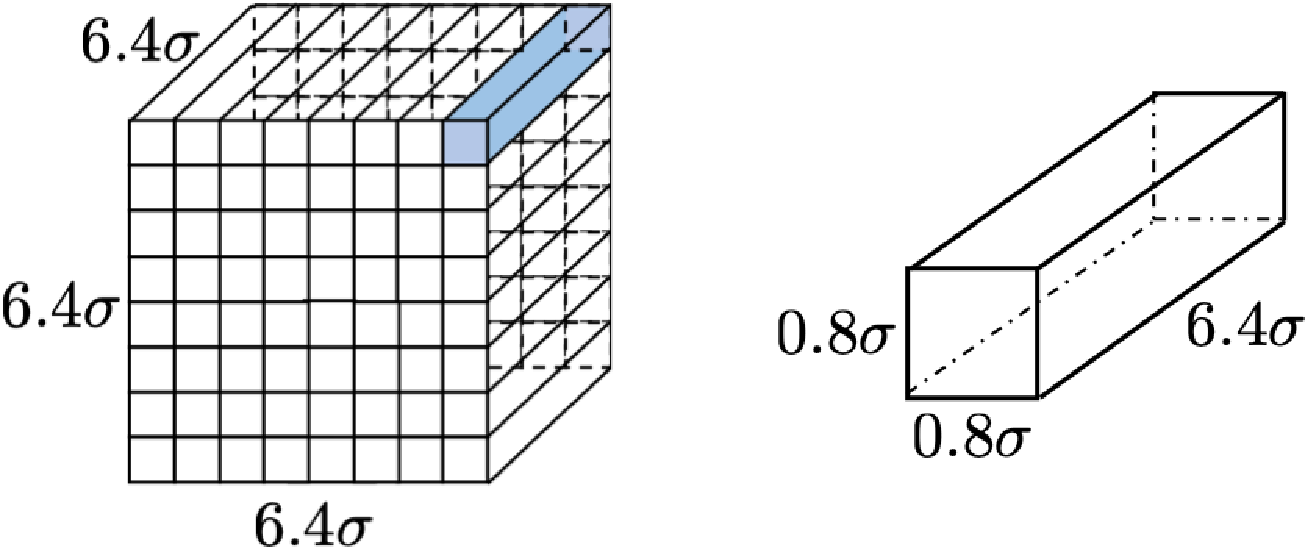
\includegraphics[scale = 0.7]{figures/box1.pdf}
\caption{シミュレーションボックスと分割した直方体}
\end{figure}
%	
%
\begin{figure}[H]
\centering
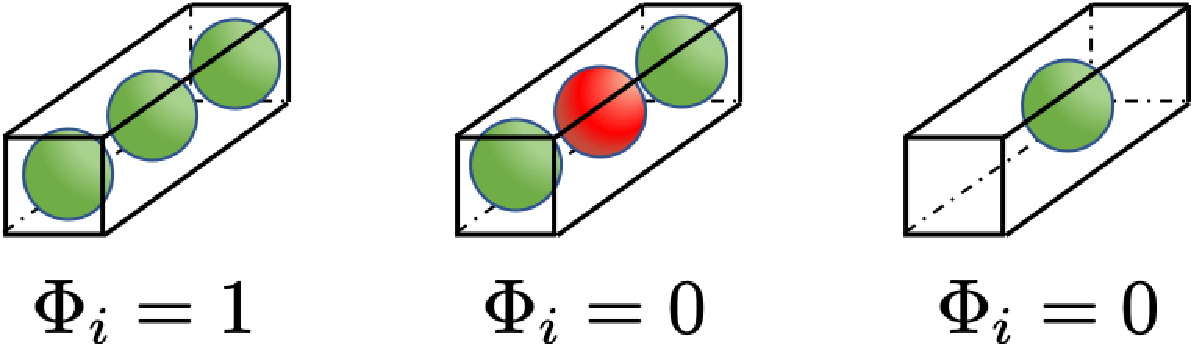
\includegraphics[scale = 0.7]{figures/box2.pdf}
\caption{レーン形成率の定義}
\end{figure}
%	
%
%
%
%
